\documentclass{article}

\usepackage[paperwidth=118.9cm,paperheight=84.1cm,margin=0cm]{geometry}
\usepackage[T1]{fontenc}
\usepackage[utf8]{inputenc}
\usepackage{lmodern}
\usepackage{graphicx}
\usepackage{xcolor}
\usepackage{tikz}
\usepackage{eso-pic}
\usepackage{booktabs}
\usepackage{tabularx}
\usepackage{array}
\usepackage{enumitem}

\usetikzlibrary{positioning,arrows.meta,shapes.geometric,calc}
\pagestyle{empty}
\setlength{\parindent}{0pt}
\setlength{\parskip}{0pt}

\definecolor{accent}{RGB}{15,76,129}
\definecolor{softblue}{RGB}{227,239,250}
\definecolor{softgreen}{RGB}{229,244,232}
\definecolor{softorange}{RGB}{253,239,220}
\definecolor{softgray}{RGB}{245,247,249}
\definecolor{softred}{RGB}{251,232,232}

\newcolumntype{Y}{>{\raggedright\arraybackslash}X}

\newcommand{\TitleFont}{\fontsize{38}{42}\selectfont\bfseries}
\newcommand{\AuthorFont}{\fontsize{20}{24}\selectfont}
\newcommand{\BodyFont}{\fontsize{18}{23}\selectfont}
\newcommand{\SmallFont}{\fontsize{15}{19}\selectfont}
\newcommand{\TinyPosterFont}{\fontsize{13}{16}\selectfont}
\newcommand{\SubHead}[1]{{\fontsize{23}{27}\selectfont\bfseries\color{accent} #1}}
\newcommand{\PosterBlock}[4]{%
  \node[anchor=north west, text width=#3, align=left] at ([xshift=#1,yshift=-#2]current page.north west) {#4};
}
\newcommand{\Pill}[2]{%
  \tikz[baseline=(n.base)]{
    \node[rounded corners=4pt, fill=#1, inner xsep=8pt, inner ysep=4pt] (n) {\bfseries\SmallFont #2};
  }%
}

\AddToShipoutPictureBG*{%
  \includegraphics[width=\paperwidth,height=\paperheight]{../../Copy of Poster Research Showcase.png}%
}

\begin{document}

\begin{tikzpicture}[remember picture,overlay]
  % Hide placeholder title/author area from the template.
  \fill[white] ([xshift=33cm,yshift=-2.8cm]current page.north west)
    rectangle ([xshift=88cm,yshift=-13.2cm]current page.north west);

  \node[anchor=north, align=center, text width=56cm] at ([yshift=-3.2cm]current page.north) {%
    {\TitleFont Nocturnal Visual Place Recognition\\[0.15cm] for Campus-Scale Robot Localization}\\[0.55cm]
    {\AuthorFont Rhoda Ojetola \hspace{0.7cm} Peter Adeyemo \hspace{0.7cm} Samuel Olusola}\\[0.2cm]
    {\AuthorFont Carnegie Mellon University Africa, Kigali, Rwanda}
  };

  % Background
  \PosterBlock{2.6cm}{17.8cm}{34cm}{%
    \BodyFont
    \begin{minipage}[t]{16.2cm}
      \centering
      
\includegraphics[width=\linewidth,height=10.7cm,keepaspectratio]{../../custom_dataset/day_images/image010.jpg}\\[0.25cm]
      \Pill{softblue}{Day reference}
    \end{minipage}\hfill
    \begin{minipage}[t]{16.2cm}
      \centering
      
\includegraphics[width=\linewidth,height=10.7cm,keepaspectratio]{../../custom_dataset/night_images/image010.jpg}\\[0.25cm]
      \Pill{softorange}{Night query}
    \end{minipage}

    \vspace{0.7cm}

    \begin{itemize}[leftmargin=1.2em,itemsep=0.35em]
      \item We study \textbf{day-to-night visual place recognition} for robot localization in GPS-denied environments.
      \item The challenge is not only illumination shift, but also \textbf{viewpoint change} and live deployment constraints.
      \item A practical system should build a map once, then localize live camera frames against it reliably.
    \end{itemize}

    \vspace{0.35cm}
    \Pill{softgreen}{Goal: recognize place from a live camera feed}
  };

  % Methodology
  \PosterBlock{2.6cm}{56.8cm}{34cm}{%
    \SubHead{Evaluation Protocol}\\[0.35cm]
    \BodyFont
    \begin{itemize}[leftmargin=1.2em,itemsep=0.3em]
      \item \textbf{Benchmark}: GardensPoint for controlled day-to-night testing.
      \item \textbf{Campus set}: 50 day reference images, 64 night queries.
      \item Metrics: \textbf{AUC}, \textbf{Recall@1/5/10}, and \textbf{Recall@100P}.
    \end{itemize}

    \vspace{0.4cm}
    \SubHead{Relabeling Insight}\\[0.25cm]
    \begin{minipage}[t]{16.3cm}
      \BodyFont
      \begin{itemize}[leftmargin=1.2em,itemsep=0.25em]
        \item Original protocol: one night image $\rightarrow$ one exact day image.
        \item New protocol: one night image $\rightarrow$ one \textbf{place ID} with multiple valid day views.
        \item This exposed that strict image-level labels were under-crediting correct same-place matches.
      \end{itemize}
    \end{minipage}\hfill
    \begin{minipage}[t]{16.0cm}
      \centering
      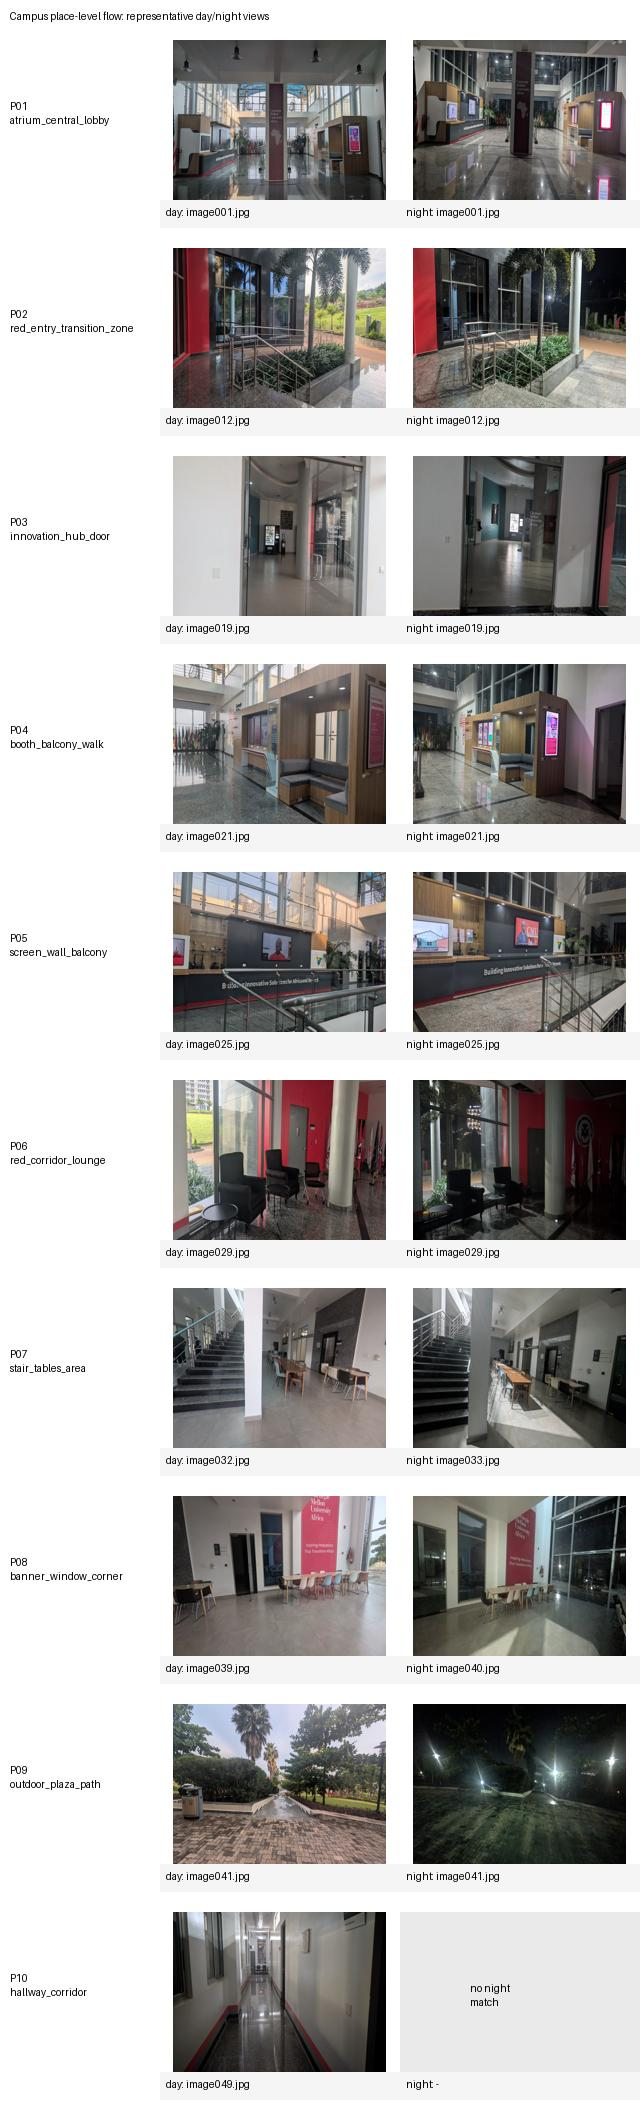
\includegraphics[width=\linewidth,height=11.2cm,keepaspectratio]{../../custom_dataset_place_level/place_flow_visual.jpg}
    \end{minipage}
  };

  % Our Solution
  \PosterBlock{42.8cm}{17.6cm}{35.6cm}{%
    \SubHead{Two-Phase VPR Pipeline}\\[0.5cm]
    \begin{center}
    \begin{tikzpicture}[
      node distance=7mm and 7mm,
      box/.style={draw, rounded corners, align=center, minimum width=8.2cm, minimum height=2.4cm, fill=softgray},
      arrow/.style={-{Latex[length=3mm]}, line width=0.9mm, accent}
    ]
      \node[box, fill=softblue] (mapsrc) {\BodyFont Day images or\\recorded traversal};
      \node[box, right=of mapsrc, fill=softgreen] (extract) {\BodyFont Descriptor extraction\\CosPlace / EigenPlaces / PatchNetVLAD};
      \node[box, right=of extract, fill=softorange] (store) {\BodyFont Saved map\\descriptors + image paths + metadata};

      \node[box, below=1.5cm of extract, fill=softblue] (query) {\BodyFont Live frame\\webcam / phone / TurboPi};
      \node[box, right=of query, fill=softgreen] (search) {\BodyFont Search backend\\Exact / HNSW / FAISS};
      \node[box, right=of search, fill=softorange] (result) {\BodyFont Top-$k$ matches\\thresholded decision\\live overlay};

      \draw[arrow] (mapsrc) -- (extract);
      \draw[arrow] (extract) -- (store);
      \draw[arrow] (query) -- (search);
      \draw[arrow] (search) -- (result);
      \draw[arrow] (store) |- (search);
    \end{tikzpicture}
    \end{center}

    \vspace{0.8cm}
    \begin{minipage}[t]{11.3cm}
      \SubHead{Map Building}\\[0.2cm]
      \BodyFont
      \begin{itemize}[leftmargin=1.2em,itemsep=0.25em]
        \item Build from image folders or a recorded traversal video.
        \item Sample frames, extract descriptors, normalize, save reusable map.
      \end{itemize}
    \end{minipage}\hfill
    \begin{minipage}[t]{11.3cm}
      \SubHead{Online Localization}\\[0.2cm]
      \BodyFont
      \begin{itemize}[leftmargin=1.2em,itemsep=0.25em]
        \item Process live frames at configurable rate.
        \item Retrieve top-$k$ candidates and apply thresholded recognition.
      \end{itemize}
    \end{minipage}\hfill
    \begin{minipage}[t]{11.3cm}
      \SubHead{Applied CV Focus}\\[0.2cm]
      \BodyFont
      \begin{itemize}[leftmargin=1.2em,itemsep=0.25em]
        \item Config-driven pipeline for demos.
        \item Works with webcam, phone webcam, and robot stream.
      \end{itemize}
    \end{minipage}

    \vspace{0.9cm}
    \begin{center}
      \Pill{softblue}{Offline map building} \hspace{0.7cm}
      \Pill{softgreen}{Live retrieval} \hspace{0.7cm}
      \Pill{softorange}{Robot-facing deployment}
    \end{center}
  };

  % Results
  \PosterBlock{82.0cm}{17.8cm}{33.8cm}{%
    \SubHead{Main Result}\\[0.35cm]
    \BodyFont
    \begin{center}
      \Pill{softred}{Original strict labels under-credited multi-view same-place matches}
    \end{center}

    \vspace{0.45cm}
    \begin{minipage}[t]{16.0cm}
      \centering
      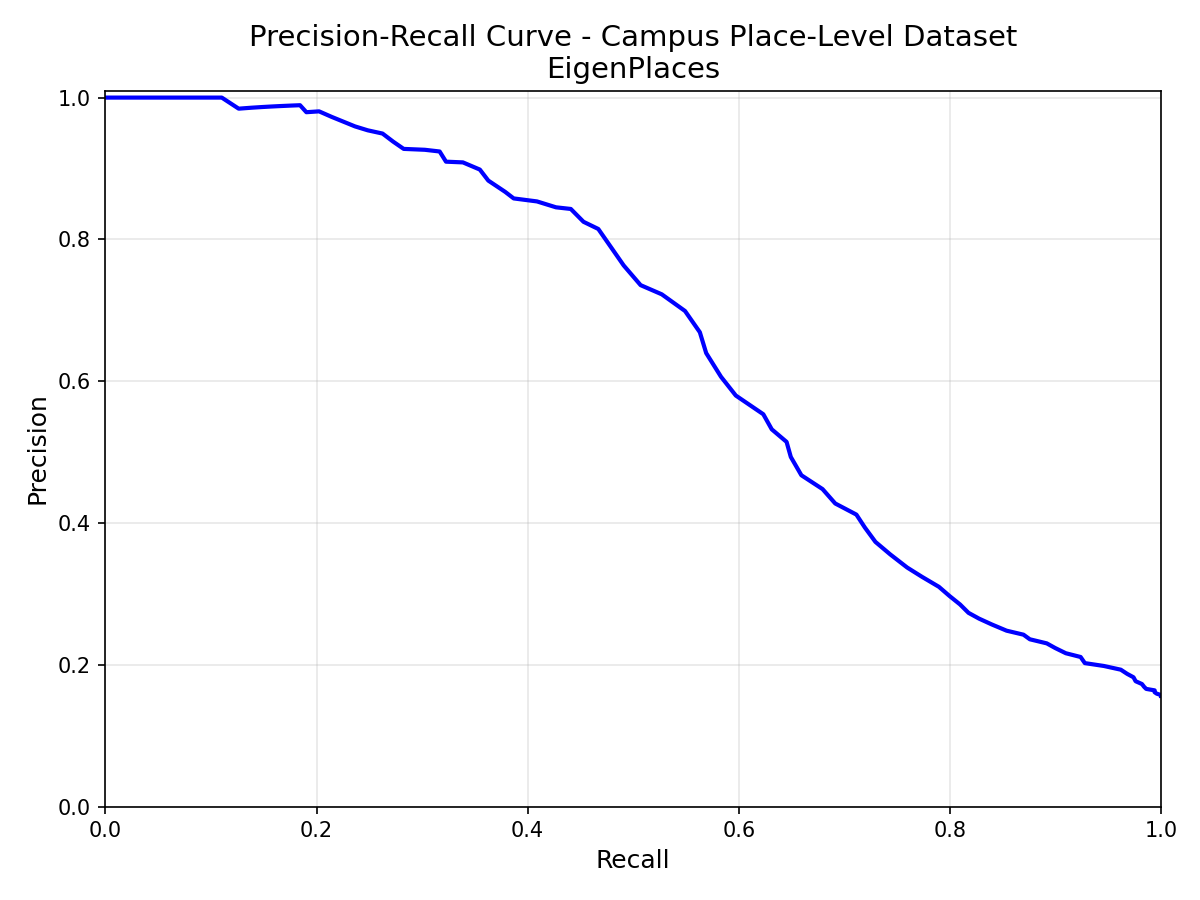
\includegraphics[width=\linewidth,height=10.6cm,keepaspectratio]{../../output_images/legacy/campus_place_level/campus_place_level_pr_curve.png}
    \end{minipage}\hfill
    \begin{minipage}[t]{16.8cm}
      \centering
      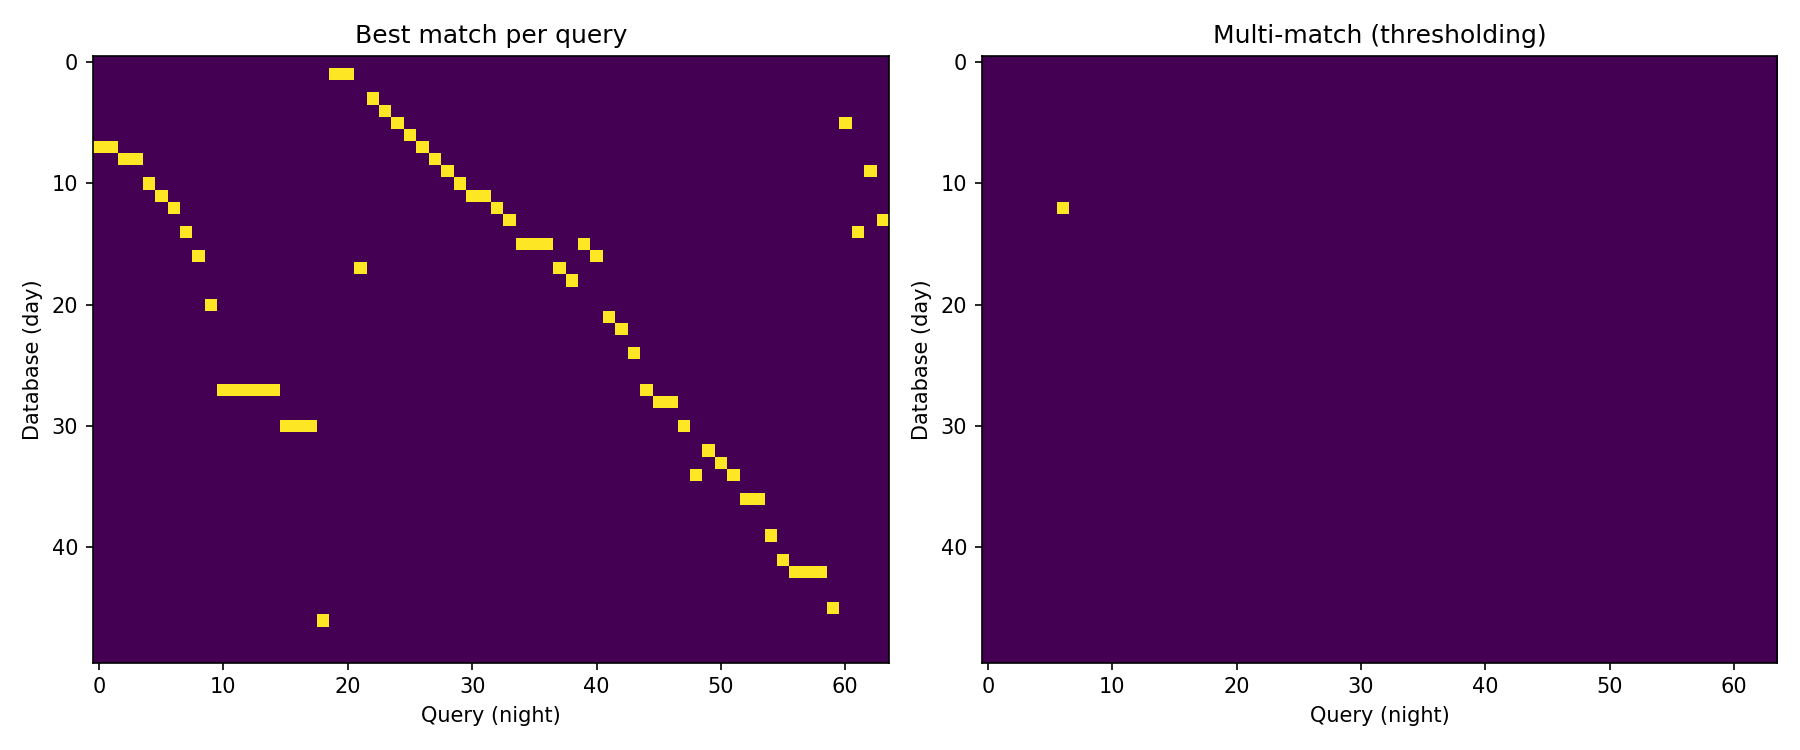
\includegraphics[width=\linewidth,height=10.6cm,keepaspectratio]{../../output_images/legacy/campus_place_level/campus_place_level_matching_results.png}
    \end{minipage}

    \vspace{0.45cm}

    {\BodyFont
    \begin{tabularx}{\linewidth}{>{\bfseries}l >{\centering\arraybackslash}p{2.8cm} >{\centering\arraybackslash}p{2.8cm} Y}
      \toprule
      Model & AUC & R@1 & Takeaway \\
      \midrule
      CosPlace & 0.627 & 0.969 & Best top-1 retrieval after place-level relabeling \\
      EigenPlaces & \textbf{0.663} & 0.922 & Best overall AUC on campus \\
      PatchNetVLAD & 0.641 & 0.938 & Strong place-level alternative \\
      HDC-DELF & 0.507 & 0.922 & Much cleaner threshold behavior \\
      \bottomrule
    \end{tabularx}
    }

    \vspace{0.45cm}
    \BodyFont
    \begin{itemize}[leftmargin=1.2em,itemsep=0.22em]
      \item Example gains after relabeling: \textbf{CosPlace R@1: 0.727 $\rightarrow$ 0.969}, \textbf{NetVLAD R@1: 0.394 $\rightarrow$ 0.891}.
      \item The original setup was not robust to multiple valid views \emph{under a strict image-level evaluation protocol}.
    \end{itemize}
  };

  % Future Research
  \PosterBlock{82.0cm}{59.0cm}{33.8cm}{%
    \SubHead{Future Research}\\[0.35cm]
    \BodyFont
    \begin{itemize}[leftmargin=1.2em,itemsep=0.35em]
      \item \textbf{Sequence-aware localization}: use temporal consistency instead of frame-by-frame decisions only.
      \item \textbf{Pose-aware filtering}: incorporate robot motion and expected observations, e.g. Kalman-filter-style prediction.
      \item \textbf{Open-set evaluation}: add a dedicated split with truly unmatched night queries after place-level review.
      \item \textbf{Robot deployment}: tighten TurboPi integration and evaluate full end-to-end live localization.
    \end{itemize}
  };

  % References
  \PosterBlock{82.0cm}{77.0cm}{33.8cm}{%
    \SubHead{References}\\[0.3cm]
    \TinyPosterFont
    \begin{enumerate}[leftmargin=1.2em,itemsep=0.2em]
      \item Berton et al., ``Rethinking Visual Geo-localization for Large-Scale Applications,'' CVPR 2022. (CosPlace)
      \item Berton et al., ``EigenPlaces: Training Viewpoint Robust Models for Visual Place Recognition,'' ICCV 2023.
      \item Arandjelovi\'c et al., ``NetVLAD: CNN Architecture for Weakly Supervised Place Recognition,'' CVPR 2016.
      \item Milford and Wyeth, ``SeqSLAM: Visual Route-Based Navigation for Sunny Summer Days and Stormy Winter Nights,'' ICRA 2012.
    \end{enumerate}
  };
\end{tikzpicture}

\end{document}
